\newpage
\hypertarget{emptyPartition vis}{}
\subsection{Implementing empty}
\visHeader

\begin{itemize}

\item[$\blacktriangleright$] Create a new activity diagram for \texttt{Partition.empty()}. To begin building the \emph{for each} pattern, quick create a new
story node and edit its properties. Name it \texttt{deleteCardsInPartition} and change its \texttt{Type} from \texttt{StoryNode} to \texttt{ForEach}. You'll
also want to create the invoking \texttt{Partition} object, \texttt{this} (Fig.~\ref{ea:sdm_foreach}). Press \texttt{OK}, and you'll see that a \emph{for each}
node is represented as a stacked node to indicate the potential for repetition.

\begin{figure}[htbp]
\begin{center}
  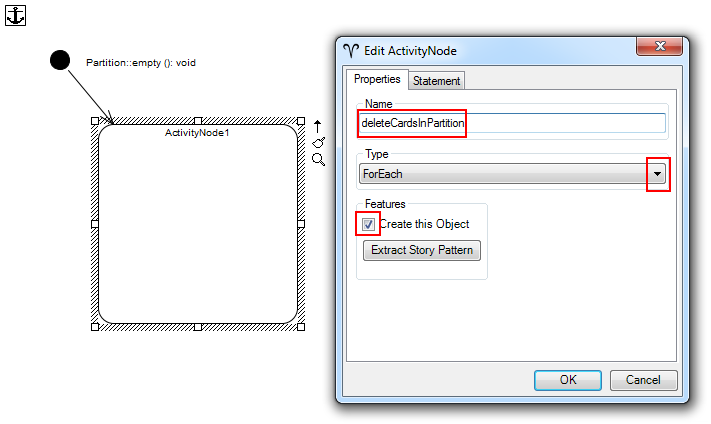
\includegraphics[width=0.9\textwidth]{ea_sdmEmptyNew}
  \caption{Creating a looping story node}  
  \label{ea:sdm_foreach}
\end{center}
\end{figure}

\item[$\blacktriangleright$] Now create the \texttt{card} object variable needed to complete this SDM. Unlike \texttt{removeCard}
(Fig.~\ref{ea:sdm_complete_control_flow}) however, the goal of \texttt{emptyCards} is not just to remove the link between the selected partition and card, we
want the matched \texttt{card} to be \emph{completely} deleted. This means in the properties tab, after setting the name and binding state, you'll need to set
the \texttt{Binding Operator} to \texttt{Destroy} (Fig.~\ref{ea:sdm_bindingOperator}).

\item[$\blacktriangleright$] Complete the story pattern as indicated in Fig.~\ref{ea:sdm_end}. Notice that the guard that terminates the looping node has an
\texttt{[end]} edge guard. Indeed, a \emph{for each} story node \emph{must} execute an \texttt{end} activity when all matches in the pattern have been
handled. \texttt{empty} is defined as a \texttt{void} method, so don't worry about setting any return value in the stop node.

\begin{figure}[htbp]
\begin{center}
  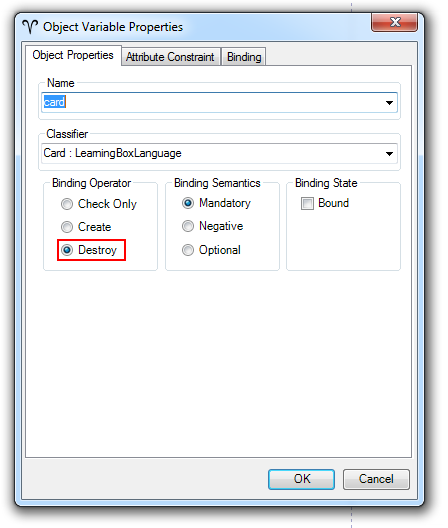
\includegraphics[width=0.65\textwidth]{ea_emptyBindingOperator}
  \caption{Editing \texttt{card} so it gets destroyed}  
  \label{ea:sdm_bindingOperator}
\end{center}
\end{figure}

\begin{figure}[htbp]
\begin{center}
  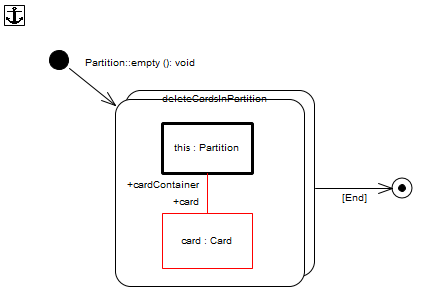
\includegraphics[width=0.8\textwidth]{ea_sdmEmptyComplete}
  \caption{Completed \texttt{empty} story pattern}  
  \label{ea:sdm_end}
\end{center}
\end{figure}
\FloatBarrier

\item[$\blacktriangleright$] Done! You've now learnt that in order to create a repeating action, all you need to do is change a standard story node
into a \texttt{for each} node, and use appropriate \emph{edge guards}. 

\vspace{0.5cm}

\item[$\blacktriangleright$] As always, save and build your metamodel. Inspect Fig.~\ref{eclipse:emptyControlFlow} and Fig.~\ref{eclipse:emptyPattern} to see
how this SDM is implemented textually.

\vspace{0.5cm}

\item[$\blacktriangleright$] Although the Learning Box GUI does not have an explicit action that invokes this SDM, feel free to extend it and see your SDM in
action!

\vspace{0.5cm}

\jumpSingle{sec:invertCard}

\end{itemize}

